\documentclass{report}

\usepackage[utf8]{inputenc} % Charakter-Kodierung
\usepackage[german]{babel} % Sprache

\usepackage[table,xcdraw]{xcolor} % Tabellen Farben
\usepackage{tabularx} % Dynamische Tabellenbreite
\usepackage{tcolorbox} % Graue Boxen
\usepackage{hyperref} % url Umgebung
\usepackage{todonotes} % Notizen
\usepackage{natbib} % Bibliographie
\usepackage{fancyhdr} % Header und Footer
\usepackage{multirow} % Multizeile
\usepackage{geometry} % Page layout
\usepackage{color} % Text Farben
\usepackage{graphicx}
\usepackage{float}
\usepackage{pdfpages}


% Page layout
\geometry{
	bottom=3.5cm,
	headheight=180pt
}

% Nummerierung der ersten Seiten verhindern
\pagenumbering{gobble}

% Bibstyle
\bibliographystyle{plain}

% Header / Footer
\fancypagestyle{plain}{
	\fancyhf{}% Clear header/footer
	\fancyhead[R]{
\includegraphics[width=4cm]{img/cau-logo-2017}} % Rechter header
	\fancyhead[L]{\leftmark} % Linker header
	\fancyfoot[R]{\thepage} % Rechter footer
	\fancyfoot[L]{
\includegraphics[width=1cm]{img/se-logo}} % Linker footer	
}
\pagestyle{plain}

\renewcommand{\headrulewidth}{0.5pt} % Unnötige Informationen der Kapitelangabe
\renewcommand{\footrulewidth}{0.2pt} % entfernen
\renewcommand{\chaptermark}[1]{\markboth{{#1}}{}}




% Zahlen für Fußnoten
\renewcommand{\thefootnote}{\arabic{footnote}}
\renewcommand{\thempfootnote}{\arabic{mpfootnote}}

%%%%% Ausfüllen %%%%%

% Gruppenname
\newcommand{\gruppenname}{HRS3-105B}

% Projektname
\newcommand{\projektname}{energy. by adesso}

% Semester
\newcommand{\semester}{SoSe19}



% Titelseite

\title{
	\vspace*{-3cm}
	Entwurfsdokumentation\\
	\projektname\\
	-\\
	\color{gray}
	Softwareprojekt \semester\\
	\gruppenname\\
	\vspace*{5mm}
	
\includegraphics[width=\textwidth]{img/logo}
}

\author{
	\begin{tabular}{r l@{\hspace{8\tabcolsep}} r} 
		Massoud Vincent & Shahriyari & \multirow{8}{*}{ 
\includegraphics{img/se-logo} } \\
		Jan-Niklas & Carstensen \\
		Tammo & Brüggemann \\
		Richard & Hanß \\
		Christoph & Fricke \\
		Felix & Rodriguez \\
		Mattis & thor Straten\\
		Malte & Clement \\
	\end{tabular}
}

\date{\today}





% Dokument

\begin{document}
	\maketitle
	
	%%%% Bitte löschen oder auskommentieren %%%%
	%%%%%%%%% Dient nur als Hilfe %%%%%%%%%%
	
	\chapter*{Tipps und Hilfen}\label{chp:tipps}
	\vspace*{-1.4cm}
	\begin{tcolorbox}
		\textbf{Information:} Dieses Kapitel und alle folgenden grauen Boxen dienen als Hilfestellungen und sollen im fertigen Dokument nicht enthalten sein. 
		%
		\\\\
		%
		Zur Versionsverwaltung während des Softwareprojekts muss \textit{Git} genutzt werden.
		Git führt Textdokumente mit unterschiedlichen Zeilenbearbeitungen automatisch zusammen.
		Wir empfehlen den Einsatz von \LaTeX~für alle Textdokumente.
		Um das Auto-Merging zu unterstützen, sollte nach jedem Satzende eine neue Zeile im Quelltext begonnen werden.
		Die .tex-Datei dieser PDF verdeutlicht dies.
		Erkennt Git, dass eine gleiche Zeile bearbeitet wurde, wird ein Konflikt auftreten.
		Dieser kann in der entsprechenden Datei von Hand mittels eines Texteditors behoben werden.
		%
		\\\\
		%
		Fußnoten\footnote{\url{https://www.se.informatik.uni-kiel.de/en}} werden für Homepages genutzt.
		Zitierungen können mittels eines \textit{cite}-Befehls gesetzt, z.B. \textit{citep}~\citep{Shaw2003WritingGoodSoftwareEngineeringesearchPapersMinitutorial}.
		%
		\\\\
		%
		Tipps zur UML-Modellierung können im SE-Wiki\footnote{\url{https://git.informatik.uni-kiel.de/ag-se/teaching-public/wikis/home}} nachgelesen werden.
		Achtet darauf, dass eure Diagramme stets lesbar (Vektor-Grafiken!) und gut strukturiert sind.
		Oftmals ist es sinnvoll ein bis zwei Sätze zusätzlich für Diagrammelemente zu formulieren.
		So können Missverständnisse ausgeschlossen werden, was einen Einfluss auf die Korrektur haben kann.
		Diagramme für unwichtige Tätigkeiten (z.B. Login / Logout, User erstellen / löschen, Passwort ändern etc.) sind nicht erforderlich.
		Achtet weiterhin darauf, dass interne Abläufe und Methodenaufrufe in den Frameworks nicht modelliert werden sollen.
		So soll z.B. das Sequenzdiagramm für das Erstellen einer Rechnung nicht interne Methoden und Abläufe des benutzten Frameworks abbilden, sondern nur diese Operationen zeigen, die Teil eures zukünftigen Codes sind.
	\end{tcolorbox}
	
	\todo[inline]{So kann eine TODO-Notiz erzeugt werden}
	
	\begin{figure}[h]
		\centering
		\missingfigure{So kann eine Placeholder-Grafik beispielsweise in den Text eingefügt werden.}		
		\caption{Beschreibung}
		\label{fig:x}
	\end{figure}
		
	%%%%%%%%%%%%%%%%%%%%%%%%%%%%%%
	
	\tableofcontents 
	
	\chapter{Einleitung}\label{chp:einleitung}
	\pagenumbering{arabic} % Nummerierung starten
	\thispagestyle{fancy}
	\section{Dokumentaufbau}\label{sec:dokumentaufbau}
Das Ziel dieses Dokuments ist die Dokumentation der Entwicklung des Onlineportals von adesso energy. 
Die enthaltenen Diagramme sollen neuen Teammitgliedern einen erleichterten Einstieg in die Struktur des Projekts ermöglichen 
und somit den Einarbeitungsprozess vor der aktiven Teilnahme an der Entwicklung verkürzen und vereinfachen.  
Außerdem können sich Mitarbeiter, die bereits am Projekt arbeiten, mit Hilfe dieser Entwurfsdokumentation einen Überblick über 
ihren aktuellen Stand und bei Unklarheiten ebenfalls über die Struktur des Projektes verschaffen.
Die frühe Planung des Zusammenspiels der einzelnen Anwendungsbereiche soll zu einem reibungslosen Ablauf 
in der tatsächlichen Entwicklung des Onlineportals führen und ermöglicht außerdem rechtzeitige Absprachen über die Funktionalität 
der Schnittstellen.
\\\\
Das Dokument besteht aus 8 Kapiteln, die jeweilen Kapitel werden im Folgenden kurz beschrieben. In Kapitel 2 präsentieren wir die Aufteilung unseres Teams in Gruppen, welche sich auf die Entwicklung der verschiedenen Anwendungsbereiche spezialisiert haben. In Kapitel 3 werden die Rest-API Endpunkte beschrieben sowie die verschiedenen DTO Datentypen erläutert. Daraufhin stellen wir in Kapitel 4 anwendungsbereichsspezifische 
Komponentendiagramme vor, welche die grobe Struktur der Anwendungsbereiche klären.
In Kapitel 5 folgt ein anwendungsbereichsübergreifendes Verteilungsdiagramm, welches die Verteilung der Komponenten auf die Hardware erläutert. 
Im 6. Kapitel befindet sich eine Sammlung von Klassendiagrammen, die wiederum die Struktur des Entwurfes 
der jeweiligen Anwendungsbereiche spezifizieren. Anschließend werden in Kapitel 7 die wichtigsten Abläufe von Methodenaufrufe aus den Klassendiagrammen in Sequenzdiagrammen dargestellt, um ein besseres Verständnis 
des Zusammenspiels der Klassen zu schaffen. Schließlich ist das letzte Kapitel das Glossar. 
In diesem können die Definitionen von Grundbegriffen des Projektes nachgeschlagen werden, welche in 
dieser Entwurfsdokumentation ohne Erläuterung verwendet werden. \newpage

\section{Zweckbestimmung}\label{sec:zweckbestimmung}
In diesem Abschnitt erklären wir kurz den Mehrwert, welchen unsere Software bietet. 
Für die Abrechnungen der Gas-,Wasser- und Stromkosten müssen Energieanbieter regelmäßig die Zählerstände ihrer
Kunden einfordern. Bisher war es Praxis diese per Post zu übermitteln oder online einzutragen. Wenn bei ersterem Fehler auftraten, musste weiterer Briefverkehr erfolgen.\\
Der Zweck des Systems ist die Vereinfachung des beschriebenen Szenarios. Der Upload von Bildern durch die App ersetzt den Briefverkehr und spart den Arbeitsaufwand für das Bearbeiten der Post ein. Administratoren können über das Back-End, an das die Kunden ihre Daten schicken, auf die Kundendaten zugreifen. Dies vermeidet Redundanzen und Fehler beim Übertragen der Daten in die Datenbank.\\
Aus Kundensicht ist die Benutzung komfortabel und einfach, da die App schlicht und funktional ist. Das Hochladen der Bilder ist einfach und erfordert nur geringe technische Kenntnisse. Außerdem ersetzen die Push-Notifications die, ansonsten per Brief geschickten, Aufforderungen den Zählerstand erneut abzulesen.



\section{Entwicklungsumgebung}\label{sec:entwicklungsumgebung}

\begin{table}[h]
	\centering
	\begin{tabularx}{\textwidth}{l l X}
		\rowcolor[HTML]{C0C0C0} 
		\textbf{Software} & \textbf{Version} & \textbf{URL} \\
		Java Development Kit & 8u144 & \url{http://www.oracle.com/technetwork/java/javase/downloads/index.html} \\
		\rowcolor[HTML]{E7E7E7} 
		Node & 12.9.0 & \url{nodejs.org/en/download/current} \\
		npm & 6.10.2 & \url{npmjs.com} \\
		\rowcolor[HTML]{E7E7E7} 
		React &16.9 &\url{reactjs.org}\\
		Create React App & 3.1.1 & \url{create-react-app.dev} \\
		\rowcolor[HTML]{E7E7E7} 
		Spring & 5.1.6 & \url{projects.spring.io/spring-framework} \\
		Docker & 19.03.1& \url{www.docker.com} \\
		\rowcolor[HTML]{E7E7E7} 
		Android SDK API&LVL 23 & \url {https://developer.android.com/studio/releases/platforms\#\ 6.0} \\
		PostgreSQL &11.4 & \url{www.postgresql.org} \\
		\rowcolor[HTML]{E7E7E7}
		Android Studio & 3.5 & \utl{https://developer.android.com/studio} \\
		Storybook & 5.1 &\url {https://storybook.js.org} \\
		
	\end{tabularx}
	\caption{Enwicklungsumgebung}
	\label{table:entwicklungsumgebung}
\end{table}
	
	\chapter{Team-Aufteilung}
	\thispagestyle{fancy}
	\begin{tabular}{ll}
 \rowcolor[HTML]{E7E7E7} 
 \textbf{Name} & \textbf{Zuständigkeit} \\ \hline
 Vincent & Verwaltung, Back-End u. CI/CD \\ 
 \rowcolor[HTML]{E7E7E7} 
 Malte & Back-End \\ 
 Mattis & Back-End \\ 
 \rowcolor[HTML]{E7E7E7}
 Felix & Back-End\\ 
 Richard & App\\ 
 \rowcolor[HTML]{E7E7E7}
 Niklas &  App \\ 
 Christoph & Website \\ 
 \rowcolor[HTML]{E7E7E7}
 Tammo & Website \\ 
\end{tabular}

\bigskip

	
	\chapter{Komponentendiagramme}\label{chp:komponentendiagramme}
	\thispagestyle{fancy}
	\begin{figure}[h]
	\centering
	\missingfigure{Komponentendiagramm}		
	\caption{Komponentendiagramm - A}
	\label{fig:komponentendiagramm-a}
\end{figure}

\begin{tcolorbox}
Die strukturelle Übersicht des zu entwickelnden Systems wird mittels Komponentendiagrammen modelliert. 
Auf jedes Diagramm muss eine textuelle Beschreibung (Fließtext mit Umbrüchen / Absätzen oder Tabelle) folgen, in der die Aufgaben der Subkomponenten beschrieben werden. 
\end{tcolorbox}

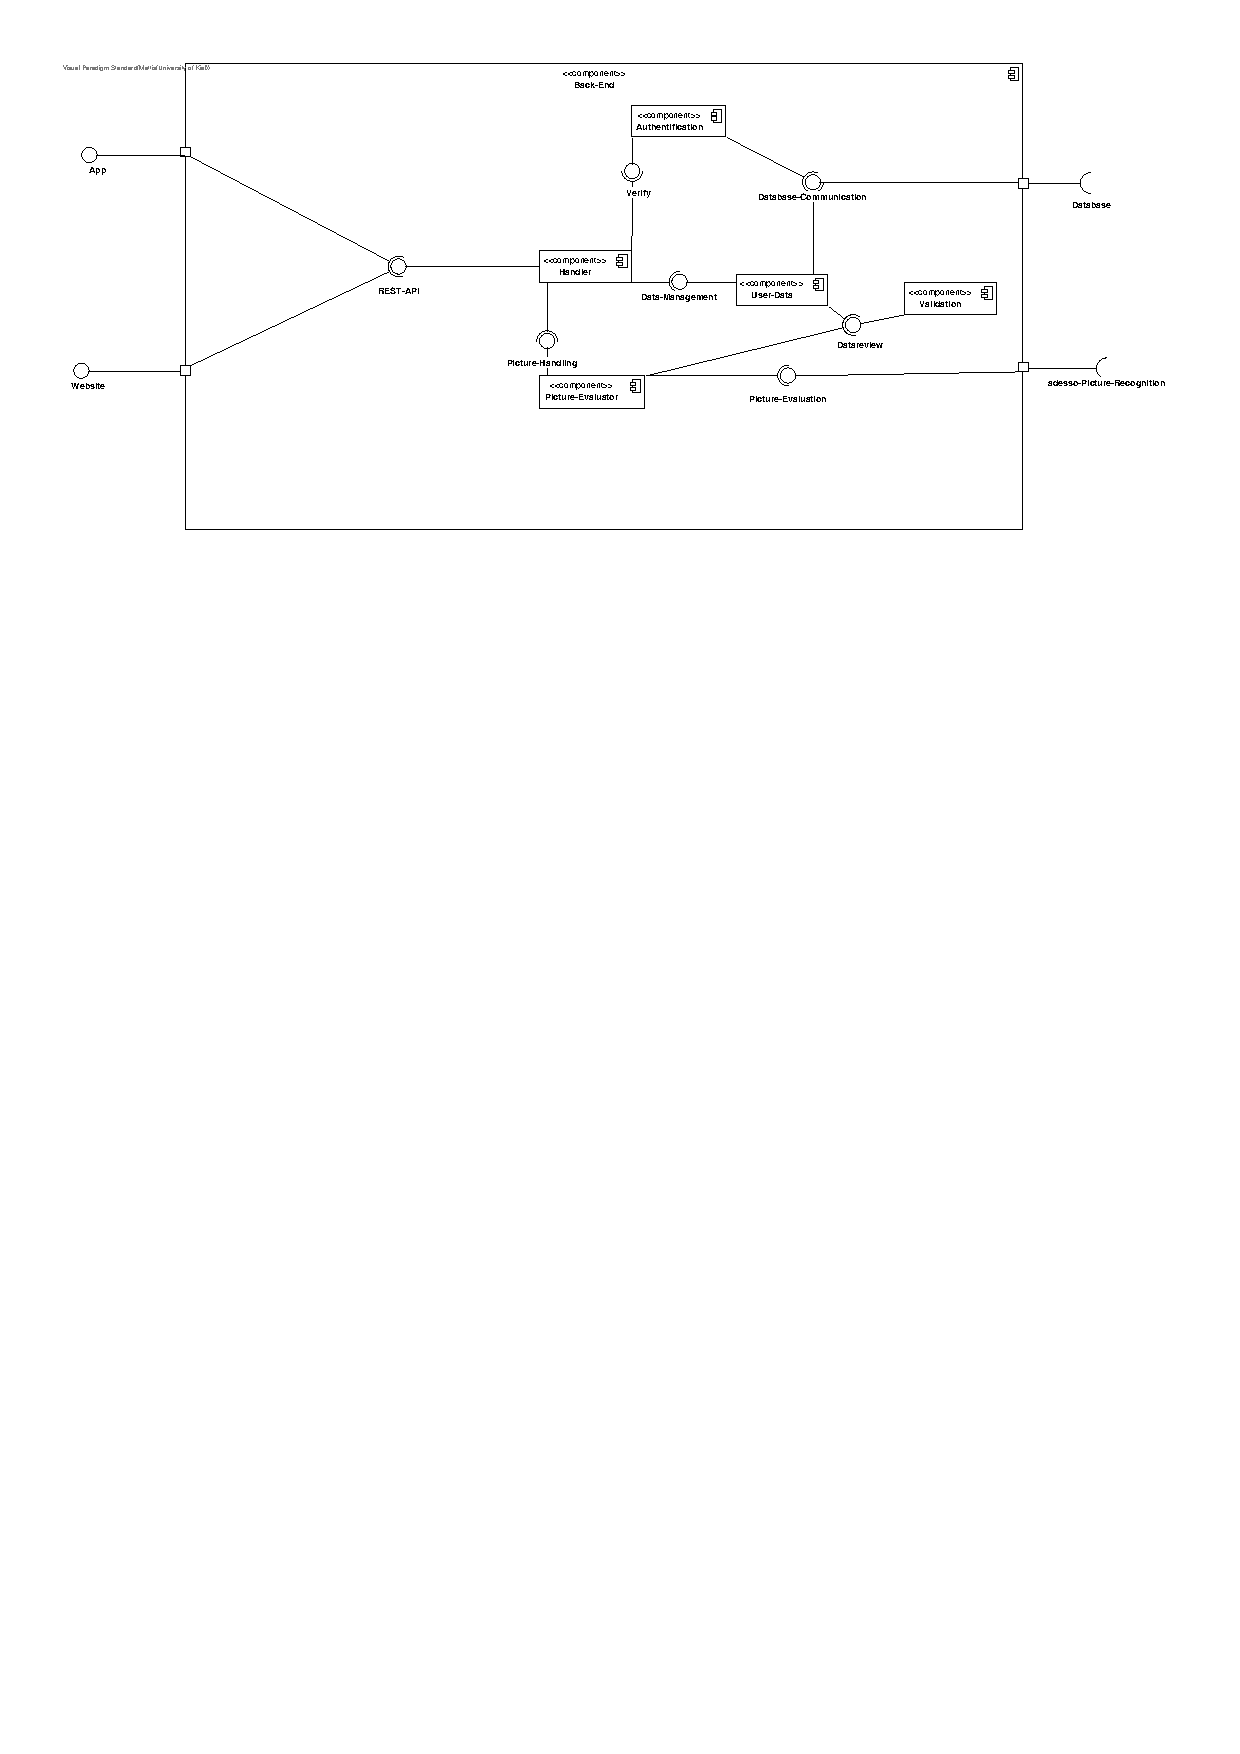
\includegraphics[scale=0.3]{\img\Komponenten_Back-Log}

Zusammengesetzt ist das "Back-End" aus mehreren Komponenenten und Schnittstellen, die untereinenander interagieren.

Dabei regelt die "Handler-Komponente" den Dateneingang durch Nutzeranfragen, indem sie die Daten an die für sie zuständigen Subkomponenten weiterleitet. Dies geschieht über die von diesen Komponenten angebotenen Schnittstellen. Die Nutzeranfragen aus App und Browser werden dabei durch die "REST-API"-Schnittstelle angenommen, welche von der "Handler"-Komponente zur Verfügung gestellt wird. 

Um zu überprüfen ob Nutzer priviligiert sind bestimmte Anfragen zu stellen existiert die "Authentification"-Komponente. Diese verhindert damit, dass Nutzer Operationen durchführen, zu welchen sie nicht befugt sind. Zu diesem Zweck stellt sie dem "Handler" eine "Verify"-Schnittstelle zur Verfügung. Um die Befugnis eines Benutzers für eine bestimmte Operation zu überprüfen, benutzt die "Authentifikation" die "Database-Communication"-Schnittstelle. Über diese werden die benötigten Rechte mit den in der Datenbank gespeicherten Rechten des Benutzers abgeglichen.

Weiterhin wird diese "Data-Communication"-Schnittstelle von der "User-Data"-Komponente genutzt. "User-Data" ermöglicht bei entsprechenden Privilegien das Abrufen oder Ändern von Kundendaten. Diese Komponente wird insbesondere genutzt um Zählerstände zu aktualisieren. 

Die gewünschten Zugriffe auf Kundendaten erfolgen über die von der "User-Data"-Komponente bereitgestellte "Data-Management"-Schnittstelle, welche von der "Handler"-Komponente verwendet wird. 

Bei Veränderungen der Daten in "User-Data" werden diese durch die "Datareview"-Schnittstelle an die "Validation"-Komponente weitergeleitet. Dort werden Zählerstände und Nummern auf ihr Format, sowie Passwörter auf Sicherheitsstandarts überprüft.

Auf die "Data-Review"-Schnittstelle greift ebenfalls die "Picture-Evaluator"-Komponente zu, um Zählernummern und Zählerstände auf Validität zu überprüfen. Diese Werte erhält die Komponenente von der "adesso-Picture-Recognition", welche die Bilder extern auswertet. Verbunden sind diese dabei über die "Picture-Evaluation"-Schnittstelle. Die Bilder welche ausgewertet werden sollen gelangen über die "Picture-Handling"-Schnittstelle, welche von der "Picture-Evaluator"-Komponente angeboten wird, in eben diese. Umgekehrt werden die daraus erhaltenen Daten über die gleiche Schnittstelle an die "Handler"-Komponente zurückgesendet. Die "Picture-Evaluator"-Komponente fungiert somit als Knotenpunkt für die Bildverarbeitung. 


	
	\chapter{Verteilungsdiagramm}\label{chp:verteilungsdiagramm}
	\thispagestyle{fancy}
	\begin{figure}[h]
	\centering
	\missingfigure{Verteilungsdiagramm}		
	\caption{Verteilungsdiagramm}
	\label{fig:verteilungsdiagramm}
\end{figure}

\begin{tcolorbox}
	Das zukünftige Deployment des Systems wird mittels einem Verteilungsdiagramm modelliert.
	Weiterhin sollten wichtige oder eventuell undeutliche Zusammenhänge (z.B. warum Schnittstelle X genutzt wird) in einem Fließtext beschrieben werden.
\end{tcolorbox}
		
	\chapter{Klassendiagramme}\label{chp:klassendiagramme}
	\thispagestyle{fancy}
	
\section{Einleitung zu den Klassendiagrammen}
In der Web-Application benutzen wir Typescript um in Javascript Typsicherheit zu gewähren. In den Diagrammen werden deshalb Typescript spezifische Typen und Utility Typen benutzt. Hierfür siehe Typescript Docs für Advanced Types und Utility Types: \\
\url{http://www.typescriptlang.org/docs/handbook/advanced-types.html} \\
\url{http://www.typescriptlang.org/docs/handbook/utility-types.html}

\begin{figure}[H]
	\hspace{-3cm}
	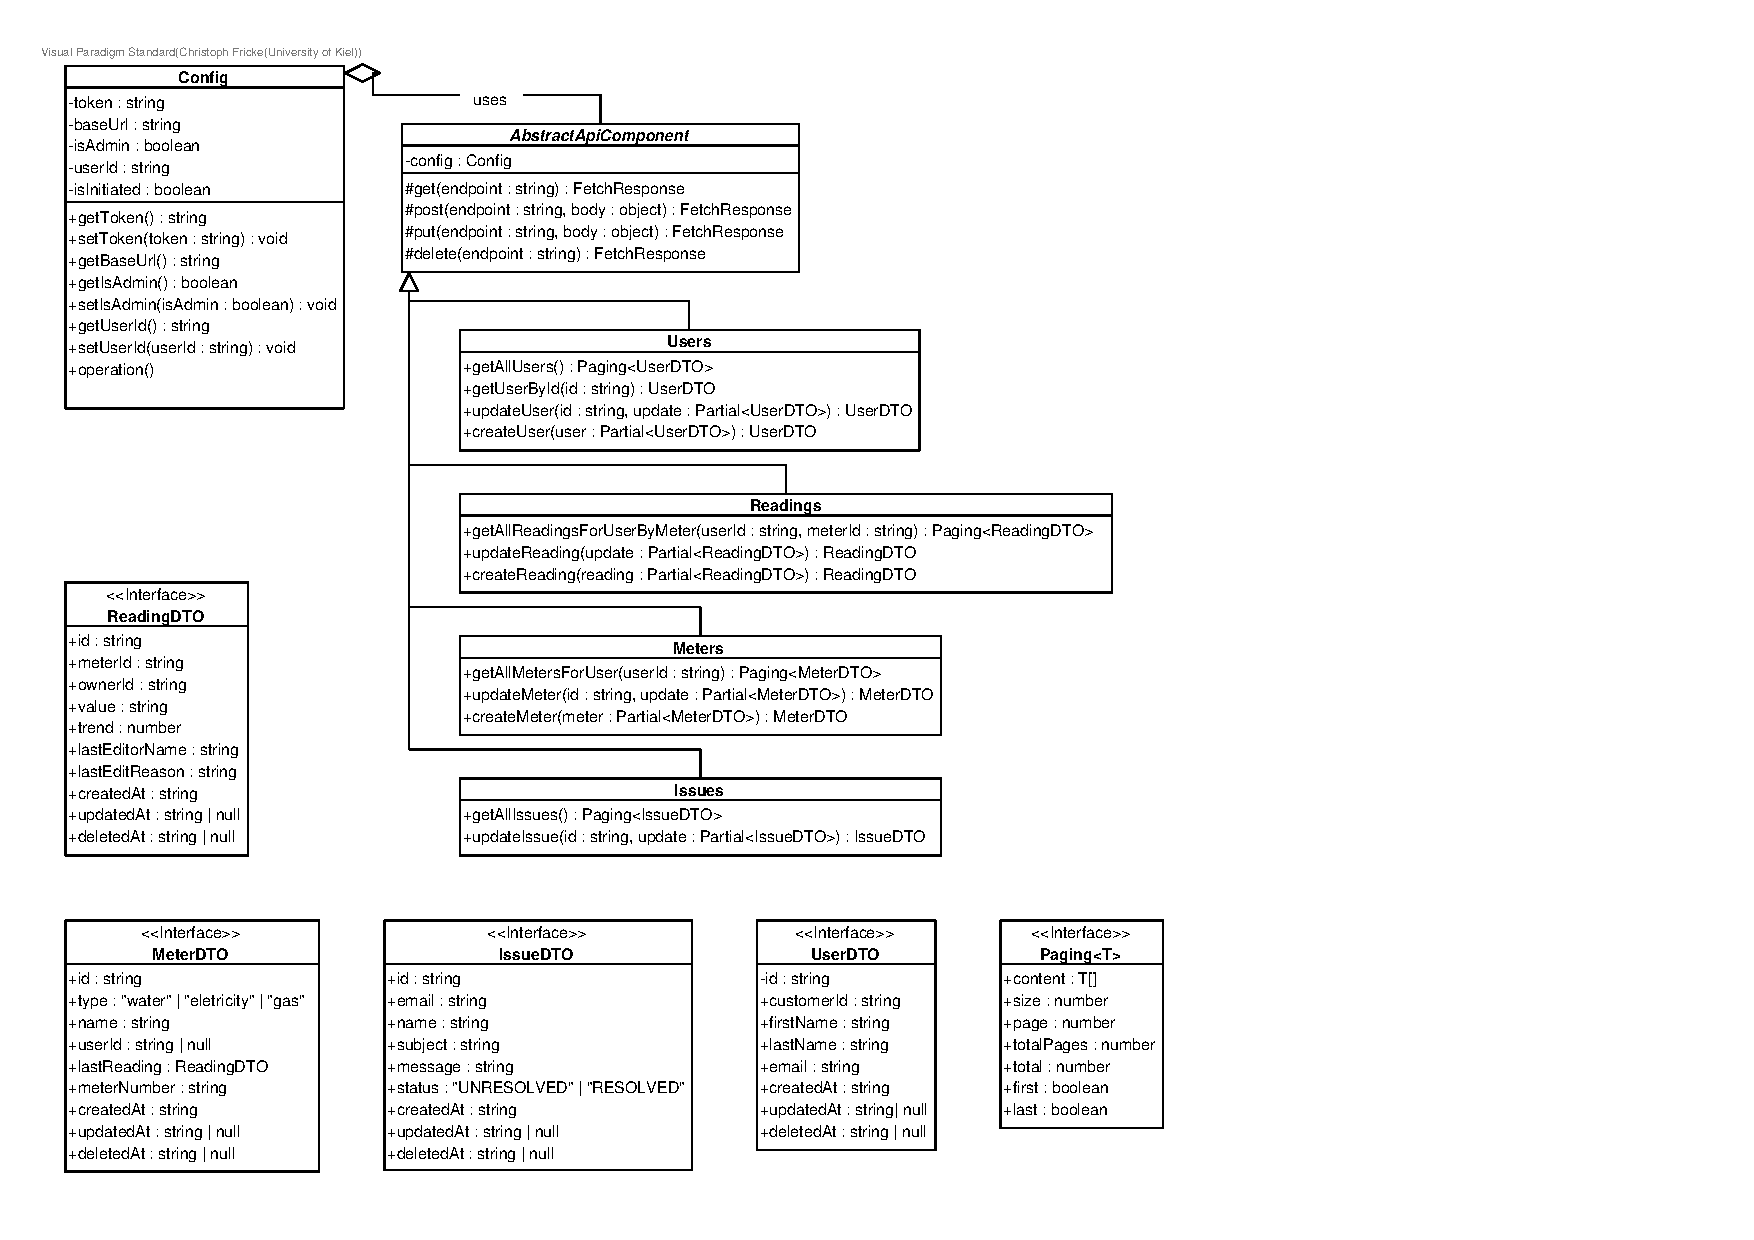
\includegraphics[scale = 0.9]{./img/diagrams/api-classDiagram}
	\caption{Klassendiagramm - API Abstraction}
\end{figure}
\newpage

\textbf{Beschreibung zum obrigen Klassendiagramm - API Abstraction.} \\ \\
Die verschiedenen DTO Interface sind Datentypen welche über die REST-Endpunkten verschickt werden. Sie dienen als Datentyp für Javascript Objekte in Typescript. In der API-Abstraction halten wir eine eigene Config-Klasse, damit Komponenten welche die Abstraction benutzen, nicht bei jedem Aufruf den Token und die Base-URL mitgeben müssen. Dadurch muss die Config nur einmal initialisiert werden, sobald der Benutzer die Website lädt. \\ \\
Eine Abstrakte Klasse stellt konfigurierte Netzwerkfunktionen für die spezialisierten Klassen zur Verfügung, sodass die Methode zum erstellen von Netzwerk Anfragen (fetch oder axios) leichter ausgetauscht werden kann. \\
Die spezialisierten API Componenten + Config sind Singletons. Eine index Datei in den API Package exportiert für
jede Klasse ein Object wodurch auf einfache Art und Weise ein Singleton Pattern in JS realisiert werden kann.
Zum Testen kann weiterhin die Klasse importiert werden, sodass z.b. von der Config in jeden Test ein neues
Objekt verfügbar ist. Dieses Verhalten wäre auch durch Mocking erreichbar, ist jedoch aufwendiger umzusetzen und erzeugt mehr Overhead. \\

\begin{table}[H]
	\centering
	\begin{tabularx}{\textwidth}{X X}
		\rowcolor[HTML]{C0C0C0} 
		\textbf{Klassenname} & \textbf{Aufgabe} \\
		Config& Speichert API Access Informationen wie Token und Base-URL. Auf diese kann nicht zugegriffen werden, bevor die Config initialisiert wurde.  \\
		\rowcolor[HTML]{E7E7E7} 
		AbstractApiComponent & Stellt konfigurierte Netzwerkfunktionen für die spezialisierten Klassen zur Verfügung. \\
		Users & Beinhaltet Funktionen um auf die Rest-Endpunkte zuzugreifen, welche inhaltlich zu den Benutzern gehören. \\
		\rowcolor[HTML]{E7E7E7} 
		Readings & Beinhaltet Funktionen um auf die Rest-Endpunkte zuzugreifen, welche inhaltlich zu den Zählerstände gehören. \\
		Meters & Beinhaltet Funktionen um auf die Rest-Endpunkte zuzugreifen, welche inhaltlich zu den Zählern gehören. \\
		\rowcolor[HTML]{E7E7E7} 
		Issues & Beinhaltet Funktionen um auf die Rest-Endpunkte zuzugreifen, welche inhaltlich zu den Tickets gehören. \\
	\end{tabularx}
	\caption{Klassenbeschreibung - API Abstraction}
	\label{table:klassenbeschreibung-api Abstraction}
\end{table}


\begin{figure}[H]
	\hspace{-3cm}
	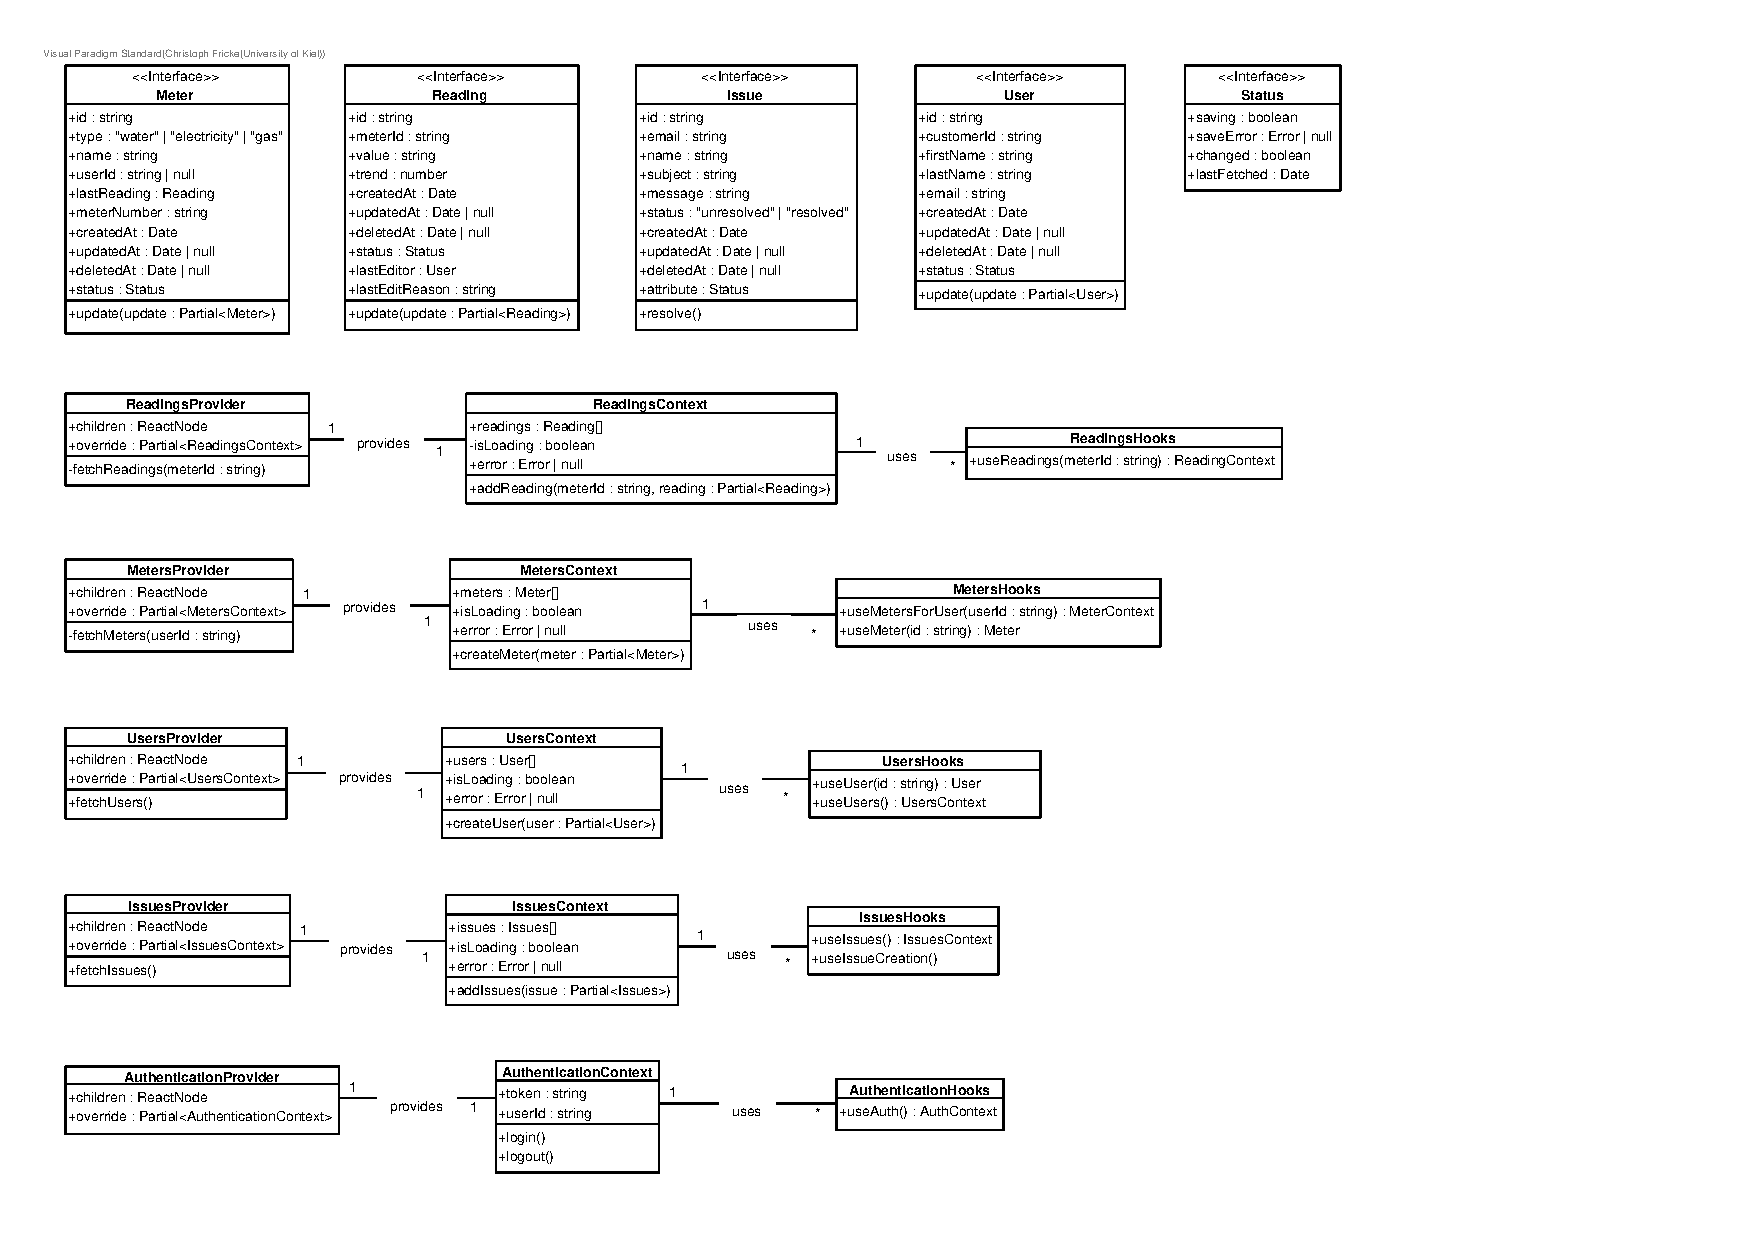
\includegraphics[scale = 0.9]{./img/diagrams/providers-classDiagram}
	\caption{Klassendiagramm - Provider}
\end{figure}
\newpage

\textbf{Beschreibung zum obrigen Klassendiagramm - Provider.} \\ \\
Für das Klassendiagramm für die Provider ist es wichtig \href{https://reactjs.org/docs/context.html}{React Context} zu verstehen.  Der Override in den Providern erlaubt es uns den Context in Tests auszutauschen. Dadurch können Components, deren Kinder oder diese selber einen Access Hook  benutzen, 
getestet werden, ohne das der Hook gemockt werden muss. \href{https://reactjs.org/docs/hooks-intro.html}{Hooks} sind eine React-Funktionalität um Logik innerhalb von Componenten zu abstrahieren und wiederzuverwenden. Ein Context wird hier als Klasse dargestellt. In Wahrheit ist es aber ein Objekt, 
welches von React verwaltet wird. Dadurch werden konsumierende Components bei Updates automatisch neu gerendert. Das Ganze ist vergleichbar mit einem Observer Pattern. \\
Die Hook Klassen existieren nur im Diagramm. Im Quellcode sind es nur die aufgelisteten Hooks, welche von den UI Components benutzt werden können um Zugriff auf die Contexte zu bekommen. Die Hooks dienen damit als Fassade, sodass die React Contexte auch durch Redux für das globale State Management ersetzt werden könnten.
Provider Components bringen die verschiedene Contexte in den React-Tree, damit diese für die Hooks in den UI Components zur Verfügung stehen.\\
Die Interface welche im Context gehalten werden, sind erweiterte DTO interface welche zusätzliche interne Informationen speichern.

\begin{table}[H]
	\centering
	\begin{tabularx}{\textwidth}{X X}
		\rowcolor[HTML]{C0C0C0} 
		\textbf{Klassenname} & \textbf{Aufgabe} \\
		*Context & Conxtexte stellen ihren zugehörige Informationen global zur Verfügung.  \\
		\rowcolor[HTML]{E7E7E7} 
		*Provider & Die Provider rendern ihren zugehörigen Context in den React-Tree. \\
		*Hooks & Hooks sind Zugriffsfunktionen als Fassade für die zugehörigen Contexte, damit die Componenten nicht direkt auf den Context zugreifen. \\
	\end{tabularx}
	\caption{Klassenbeschreibung - Provider}
	\label{table:klassenbeschreibung-provider}
\end{table}
\newpage

\begin{figure}[H]
	\hspace{-3cm}
	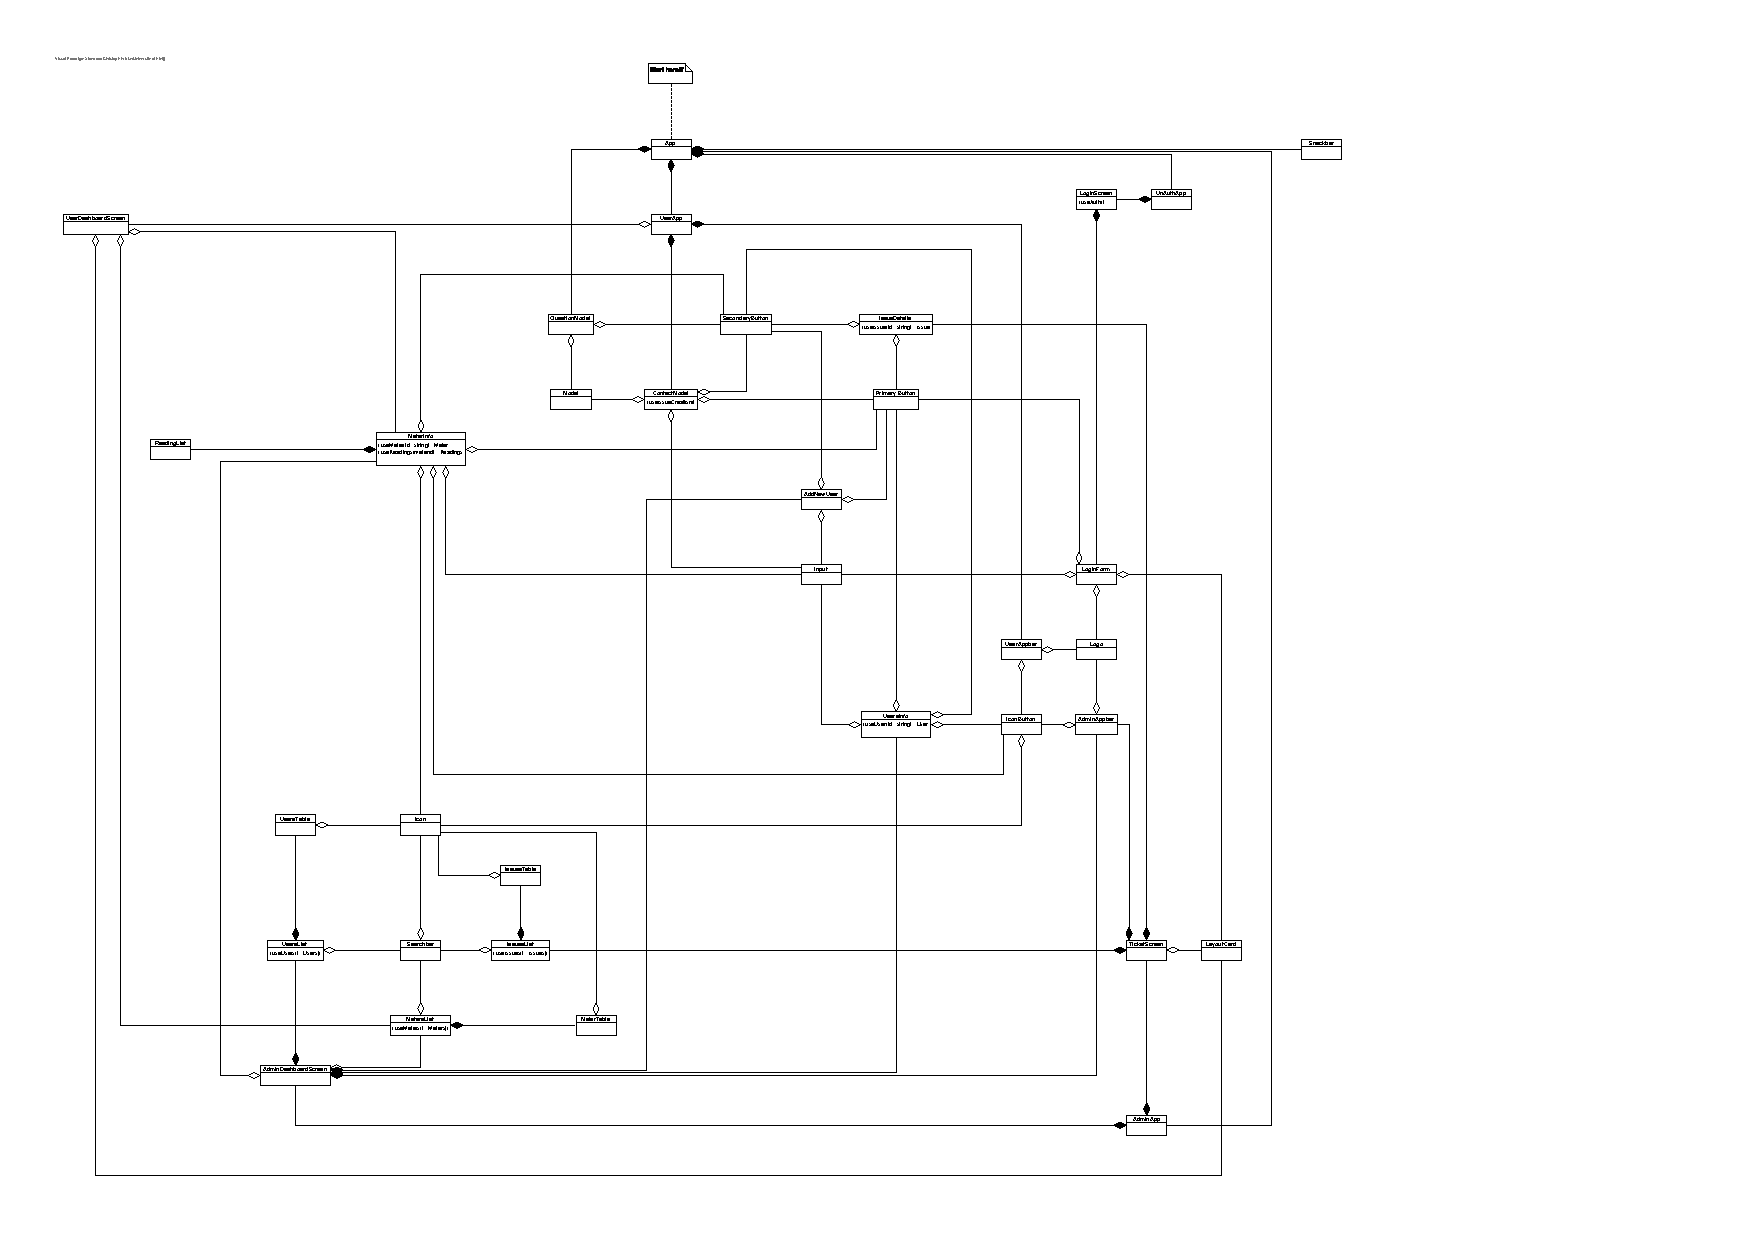
\includegraphics[scale = 0.9]{./img/diagrams/web-class}
	\caption{Klassendiagramm - Benutzeroberfläche Componenten}
\end{figure}
\newpage

\textbf{Beschreibung zum obrigen Klassendiagramm - Benutzeroberfläche Componenten} \\ \\
Alle Klassen aus dem Diagramm sind \href{https://reactjs.org/docs/components-and-props.html}{React-Componenten}. Damit es übersichtlicher ist, haben wir die Properties und internen State sowie die Kardinalitäten der Associationen rausgelassen und nur Hooks aus der Provider-Schicht hinzugefügt wo wir vermuten auf den globalen State zuzugreifen. \\ \\
Allgemein bestehen die Benutzeroberflächen aus Kompositionen von UI Componenten welche von React in den HTML-DOM gerendert werden. 
 
\begin{table}[H]
	\centering
	\begin{tabularx}{\textwidth}{X X}
		\rowcolor[HTML]{C0C0C0} 
		\textbf{Klassenname} & \textbf{Aufgabe} \\
		App & App ist die Hauptkomponente welche in den HTML-DOM gerendert wird. Basierend auf den Status des Benutzers, rendert diese entweder die 	User-App, die Admin-App oder die Unauth-App. \\
		\rowcolor[HTML]{E7E7E7} 
		Layout Card & Die Layout Card rendert eine weiße Box welche als Container für ihre inneren Componenten dient.  \\
		Snackbar & Die Snackbar sind kleine Pop-up Benachrichtigungen welche dem Benutzer Statusmeldungen mitteilen.  \\
		\rowcolor[HTML]{E7E7E7} 
		UsersList & Die UsersList rendert eine Liste mit Suchbar von allen Benutzern. \\
		MetersList & Die MetersList rendert eine Liste mit Suchbar von allen Zählern eines Benutzers. \\
		\rowcolor[HTML]{E7E7E7} 
		IssuesList & Die IssuesList rendert eine Liste mit Suchbar von allen Tickets.\\
		UsersInfo & Enthält Informationen über die Benutzer und die Möglichkeit diese zu editieren. \\
		\rowcolor[HTML]{E7E7E7} 
		IssueDetails & Enthält eine Detaillierte Ansicht über ein Ticket und Interaktions möglichkeiten.\\
		MeterInfo & Enthält Informationen über einen Zähler und seine Zählerstände.
	\end{tabularx}
	\caption{Klassenbeschreibung - Benutzeroberfläche Componenten}
	\label{table:klassenbeschreibung-ui}
\end{table}

Alle Klassen aus dem Diagramm sind \href{https://reactjs.org/docs/components-and-props.html}{React-Componenten}. Damit es übersichtlicher ist, haben wir die Properties und internen State sowie die Kardinalitäten der Associationen rausgelassen und nur Hooks aus der Provider-Schicht hinzugefügt wo wir vermuten auf den globalen State zuzugreifen. \\ \\
Allgemein bestehen die Benutzeroberflächen aus Kompositionen von UI Componenten welche von React in den HTML-DOM gerendert werden. 
 
\begin{table}[h]
	\centering
	\begin{tabularx}{\textwidth}{X X}
		\rowcolor[HTML]{C0C0C0} 
		\textbf{Klassenname} & \textbf{Aufgabe} \\
		App & App ist die Hauptkomponente welche in den HTML-DOM gerendert wird. Basierend auf den Status des Benutzers, rendert diese entweder die User-App, die Admin-App oder die Unauth-App. \\
		\rowcolor[HTML]{E7E7E7} 
		Layout Card & Die Layout Card rendert eine weiße Box welche als Container für ihre inneren Componenten dient.  \\
		Snackbar & Die Snackbar sind kleine Pop-up Benachrichtigungen welche dem Benutzer Statusmeldungen mitteilen.  \\
		\rowcolor[HTML]{E7E7E7} 
		UsersList & Die UsersList rendert eine Liste mit Suchbar von allen Benutzern. \\
		MetersList & Die MetersList rendert eine Liste mit Suchbar von allen Zählern eines Benutzers. \\
		\rowcolor[HTML]{E7E7E7} 
		IssuesList & Die IssuesList rendert eine Liste mit Suchbar von allen Tickets.\\
		UsersInfo & Enthält Informationen über die Benutzer und die Möglichkeit diese zu editieren. \\
		\rowcolor[HTML]{E7E7E7} 
		IssueDetails & Enthält eine Detaillierte Ansicht über ein Ticket und Interaktions möglichkeiten.\\
		MeterInfo & Enthält Informationen über einen Zähler und seine Zählerstände.
	\end{tabularx}
	\caption{Klassenbeschreibung - Benutzeroberfläche Componenten}
	\label{table:klassenbeschreibung-ui}
\end{table}
 
\section{Klassendiagramme - Back-End}
\begin{figure}[H]
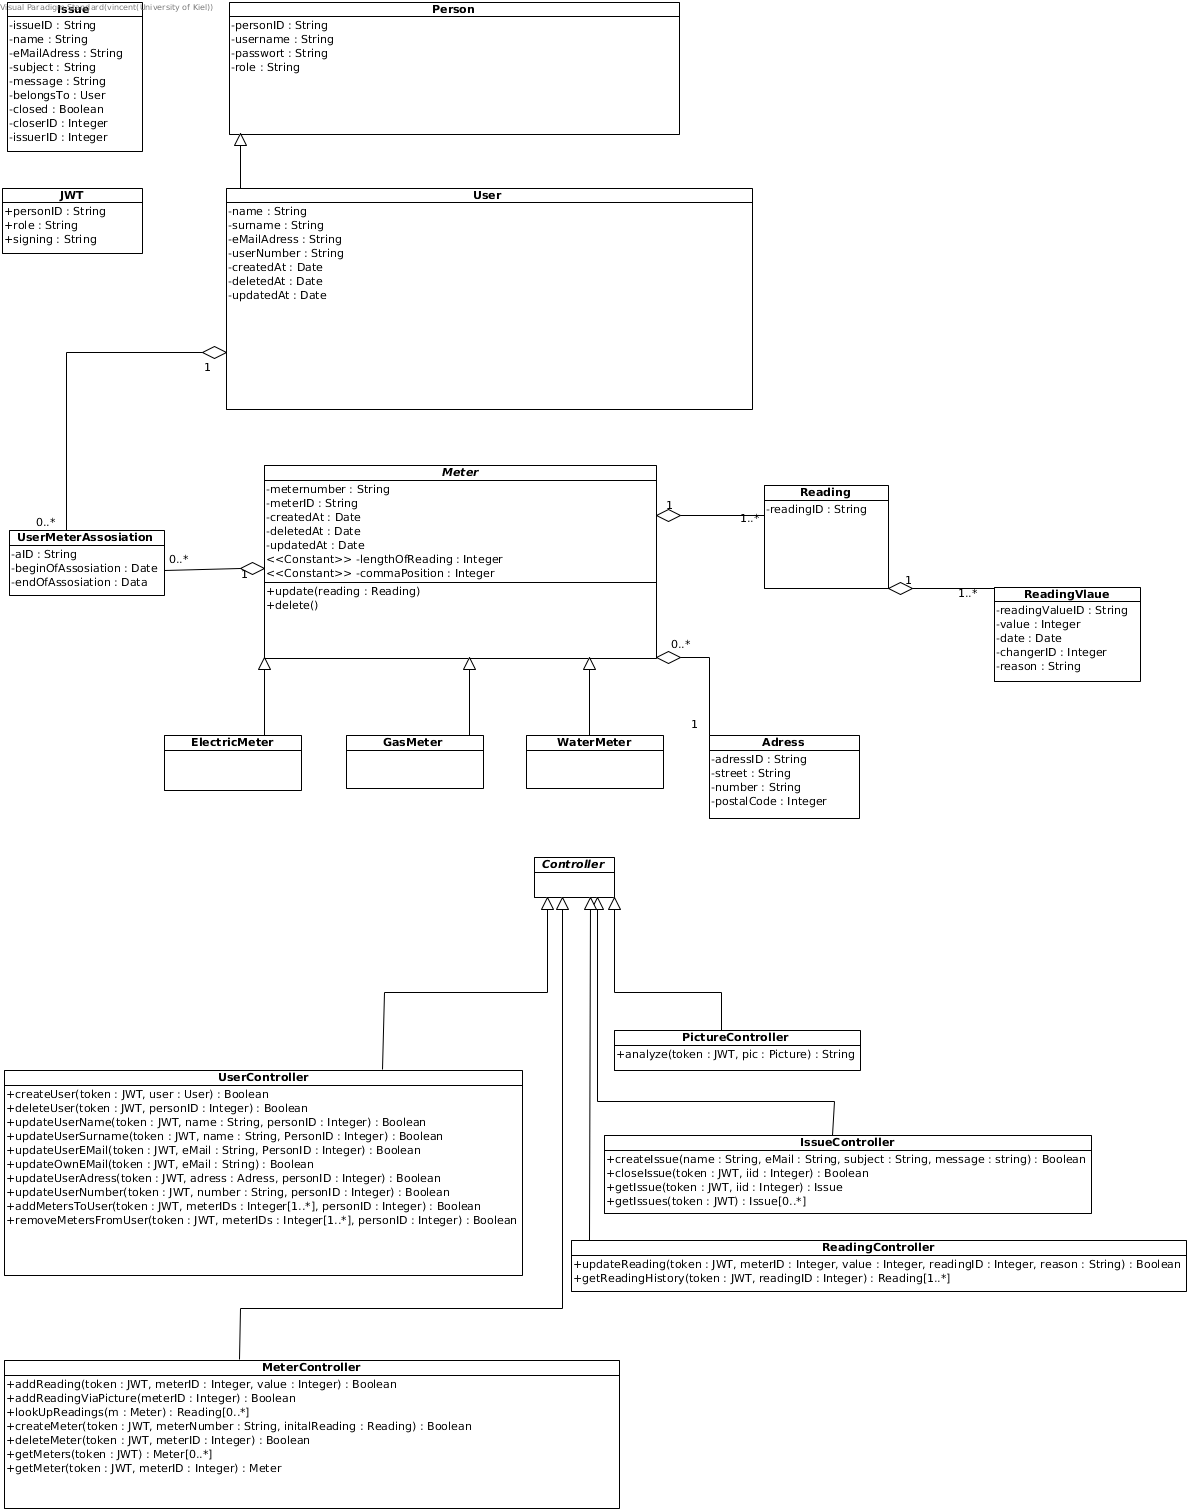
\includegraphics[width=15cm]{img/diagrams/backend-class-diagram}\\
\caption{Klassendiagramm - Back-End}
\end{figure}
Bei allen Objekten, die Entities des Models darstellen (Person, User, UserMeterAssociation, Meter, Reading, ReadingValue, Adress, Issue), handelt es sich um Spring Entity-Objekte.
Die normalerweise anfallenden Klassen (z.B. Repository-Klassen) werden zwar generiert, aber zu Übersichtszwecken nicht im Diagramm aufgeführt.\\
JWT steht für JSON Web Token. 
JWTs werden genutzt, um bei Anfragen an die REST-API User und Administratoren zu authentifizieren. Die REST-API wird durch den Controller bereitgestellt.
Man kann daher auch aus jeder Anfrage, die einen JWT enthält, einen konkreten User herauslesen. 
Da es sich um ein JSON-Objekt handelt, wird es intern nur als String wahrgenommen, aber zur Übersicht im Diagramm wurde es mit dem geplantem Inhalt als Java-Klasse aufgeführt.\\
Da Kunden aus einer Wohnung ausziehen können und neue Kunden dort einziehen können, benötigen Kunden und Zähler eine Komponente oder Funktion, welche einen Zähler zu einem Gewissen Zeitpunkt einem Kunden zuordnet. 
Zu diesem Zweck existiert die UserMeterAssosiation.\\
Ein Zähler besitzt mindestens einen aktuellen Zählerstand und gegebenenfalls mehrere alte Zählerstände, sowie eine Adresse, an der er montiert ist.\\
Das Attribut lengthOfReading wird von den konkreten Zählern geerbt und beschreibt, welche Länge eine Eingabe dieser Zählerart besitzt. Das Attribut commePosition besagt dabei, wie viele Nachkommastellen es gibt.\\
Ein Zählerstand hat mindestens einen Wert der beim Ablesen angegeben wird. 
Da er aber unter Umständen von Administratoren geändert werden kann, werden zusätzlich alle Versionen des Zählerstandes inklusive der Person die ihn verändert hat, ebenfalls wird der Grund für die Änderung gespeichert.
Beim Erstellen eines Zählerstandes wird ein ReadingValue aus dem tatsächlichen Stand des Zählers und Default-Werten für Grund und Ersteller generiert.\\
Die Controller dienen zum Auslesen und Manipulieren der Daten des Models. 
Die Controller sind jeweils darauf spezialisiert die Anfragen von Nutzern, Zählern oder Einträgen zu händeln.

\section{Klassendiagramme - App}
Die App ist intern in eine View- und eine Model/Controller-Komponente aufgeteilt. Es folgen Klassendiagramme für die 2 Komponenten.
\begin{figure}[H]
\centering
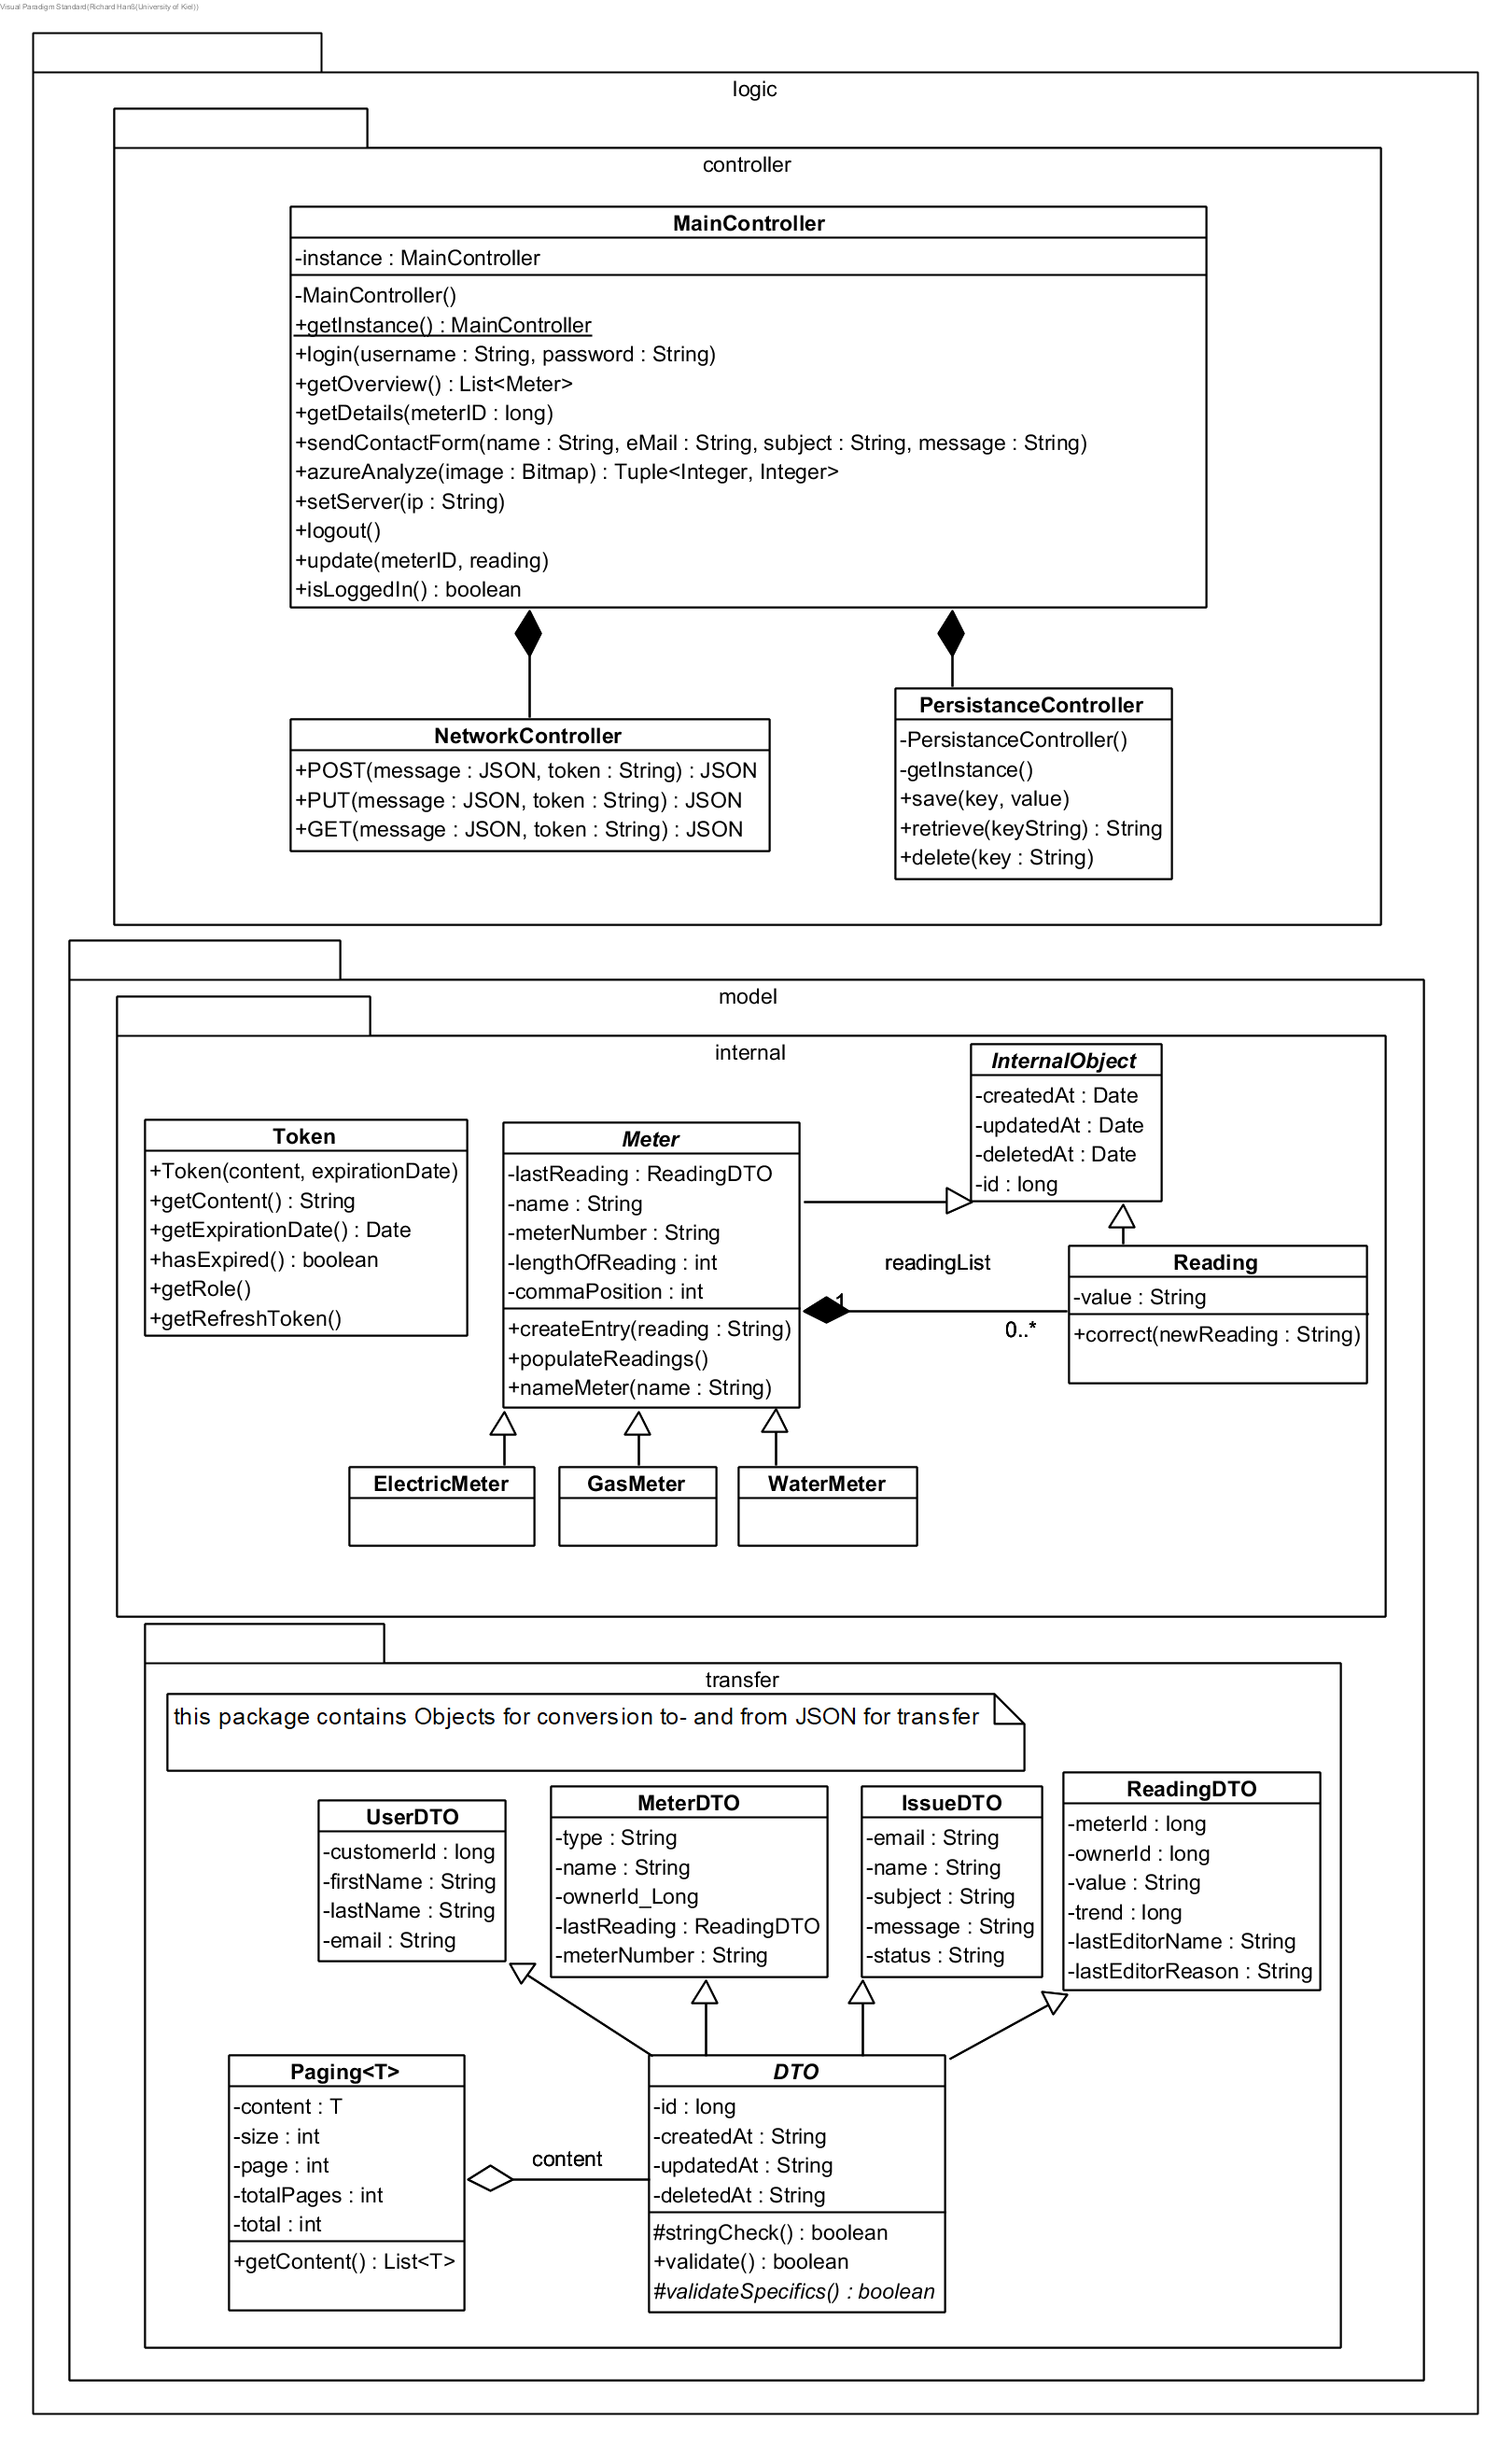
\includegraphics[scale=1.05]{img/diagrams/Android-Class-Diagram-Logic}\\
\caption{Logik der App}
\end{figure}


\subsection*{Erklärung - Model \& Controller der App}
Im Package 'logic' befinden sich die Packages 'model' und 'controller'.
Klassen im Controller-Package sind verantwortlich fürs tatsächliche Ausführen der Operationen, die vom User über Interaktion mit den Views gestartet werden. \\ Die Singleton-Klasse MainController ist hier erster Ansprechpunkt für die Views und stellt Methoden zum Ein- und Ausloggen, Analysieren von Bildern, Fetchen von Zählern, Senden von Kontaktanfragen und ändern vom zu benutzendem Server. \\ Der MainController benutzt zum senden von HTTP-Requests den NetworkController und zum Speichern von persistenten Daten (wie z.b. OAuth Token) den PersistanceController.
Das Model ist in 2 Packages unterteilt. 'internal' enthält Objekte, die den Views zur Anzeige übergeben werden, sowie eine Repräsentation des OAuth-Tokens. \\ Im 'transfer' package befinden sich Klassen, die identisch zu den über REST zu übertragenden JSON Objekten aufgebaut sind. Sie werden über eine Library von- und zu JSON konvertiert werden.

\begin{figure}[H]
\hspace{-1cm}
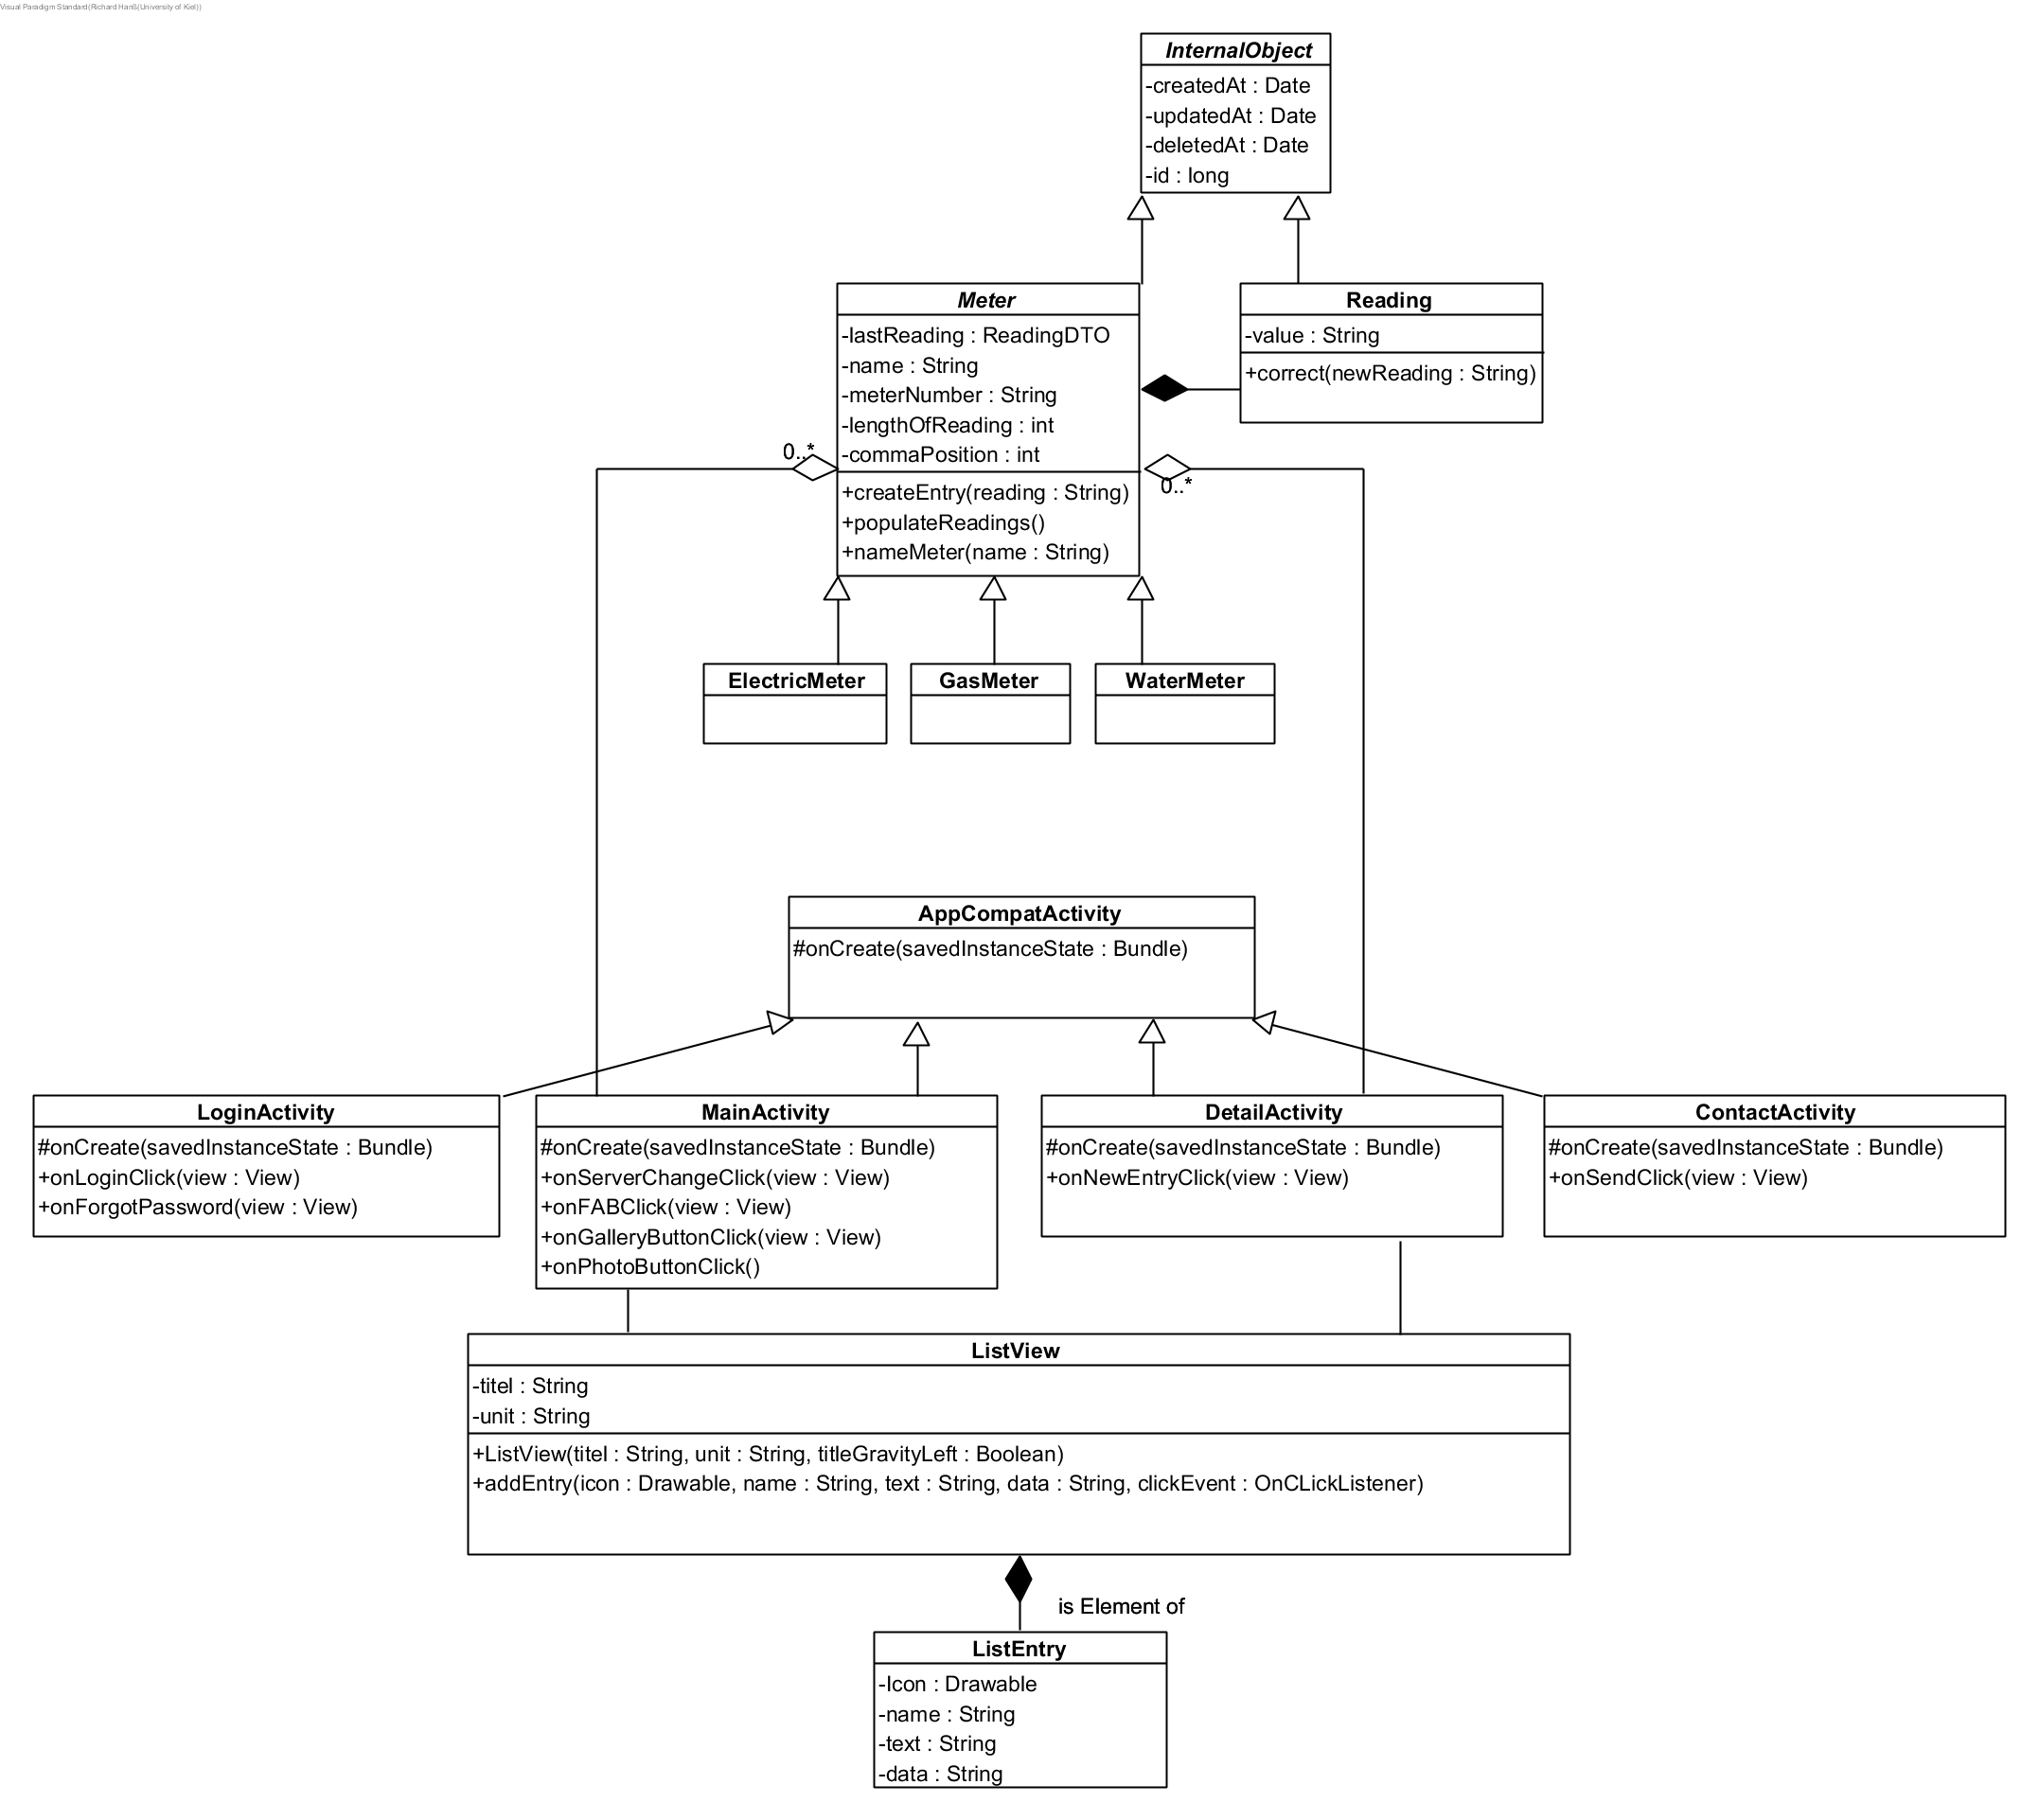
\includegraphics[scale=0.95]{img/diagrams/Android-Class-Diagram-View}\\
\caption{Android View}
\end{figure}

\newpage

\subsection*{Erklärung - View der App}
\begin{tabularx}{15cm}{XX}
	\hline
	Meter/InternalObject/Reading & Die hier aufgeführte Meter Klasse ist dieselbe, die auch in dem Logikdiagram dargestellt ist. \\ \hline
	ElectricMeter/GasMeter/WaterMeter & Die hier aufgeführte Meter Klasse ist dieselbe, die auch in dem Logikdiagram dargestellt ist. \\ \hline
	AppCompatActivity & Diese Klasse ist standartmäßig die Superklasse von allen Activities in Android Studio \\ \hline
	LoginActivity & Diese Activity stellt UI Elemente bereit, die es dem Nutzer erlauben sich anzumelden. \\ \hline
	MainActivity & Auf dieser Activity kann der Nutzer seine Zähler und einige Zählerstände einsehen, sowie auf sie zugreifen. \\ \hline
	DetailActivity & Auf dieser Activity kann der Nutzer Zählerstände hinzufügen und einsehen. \\ \hline
	IssueActivity & Auf dieser Activity kann der Nutzer einen Admin kontaktieren, falls er ein Problem hat. \\ \hline
	ListView & Diese Klasse erleichtert das hinzufügen und maintainen von Listen in der ManActivity und DetailActivity. \\ \hline
	ListEntry & Diese Klasse stellt einen Listeneintrag dar. 
\end{tabularx}
	
	\chapter{Sequenzdiagramme}\label{chp:sequenzdiagramme}
	\thispagestyle{fancy}
	
In diesem Kapitel sind die Sequenzdiagramme beschrieben, die Vorgänge beschreiben bei denen das Verhalten nicht trivial ist.
Nicht trivial ist ein Verhalten, bei dem das Diagramm nicht einem ``Durchreichen'' von Aufrufen entspricht.
\section{Triviale Abfrage}
\begin{figure}[H]
	\centering
	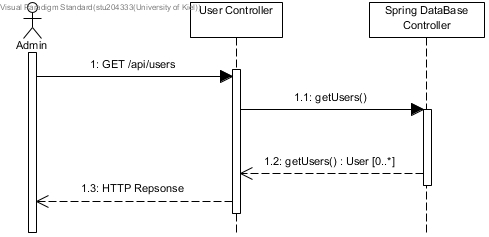
\includegraphics[width = 12cm]{img/diagrams/TrivialDiagram}
	\caption{Abfrage der Nutzerlisten}
\end{figure}
Als Beispiel für ein triviales Sequenzdiagramm lässt sich das Abfragen der Daten durch einen Admin hernehmen. Dabei beschreibt ``User [0..*]'' die Rückgabe eines ``UserList DTO''.
 
\section{Bilder in der App übermitteln}
\begin{figure}[H]
	\centering
	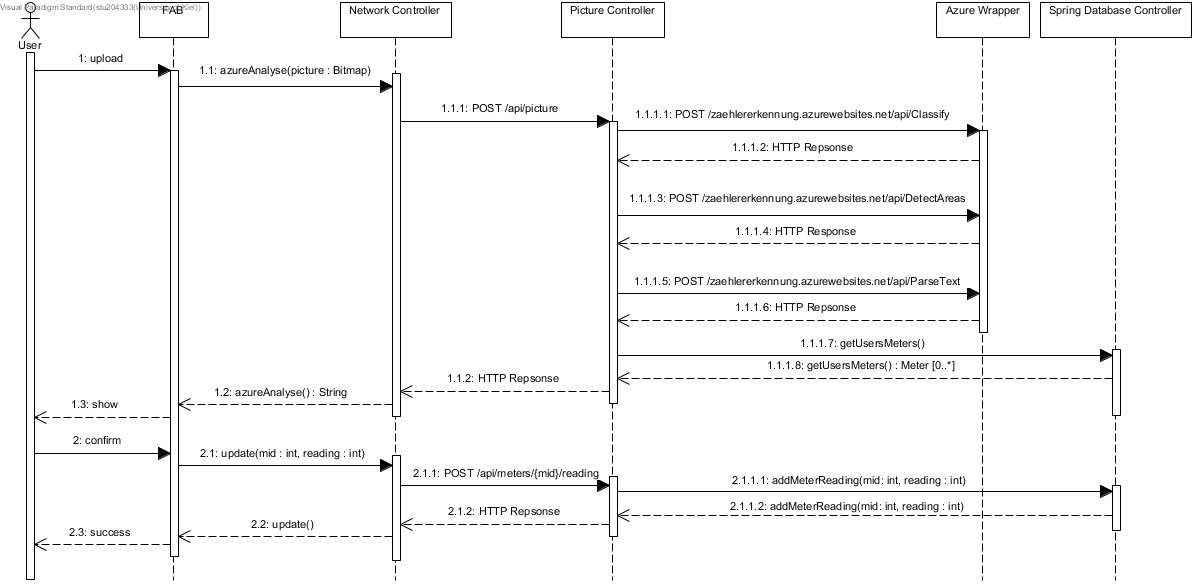
\includegraphics[width=16cm]{img/diagrams/SubmitFotoSequence}
	\caption{Erfolgreiche Bildübermittlung}
\end{figure}
Das folgende Sequenzdiagramm beschreibt den Vorgang des erfolgreichen Übermittelns eines Zählerstandes als Bild.Zuerst lädt der Nutzer ein Foto hoch, dieses wird mittels der Methode azureAnalyse vom Netzwerk-Controller per POST-Request ans Backend der Website geschickt. Dieses leitet das Bild per HTTP an die Klassifizierungsschnittstelle des AzureWrappers weiter. Nach der Antwort wird über HTTP das Bild an die nächste Schnittstelle Area-Detect geschickt. Als letztes wird das Bild noch per HTTP an die Schnittstelle Parse-Text geschickt. Die erhaltenen Daten werden jetzt einer ersten Plausibilitätsprüfung unterzogen. (Richtigkeit der Stellen und Klassifizierung)\\
Nun werden mittels getUsersMeters() alle Zähler für den Nutzer von der Datenbank abgefragt, um zu Prüfen, ob die Nummer des Zählers der Nummer eines der Zähler des Users entspricht.
Wenn dies der Fall ist, wird eine HTTP Response an den Network-Controller gesendet, die die gelesene Zählernummer und den gelesenen Zählerstand übermittelt. Nun wird der Nutzer aufgefordert die gelesenen Werte zu bestätigen. \\
Die Bestätigung entspricht dabei einer manuellen Eingabe.\\
Der Ablauf eines manuellen Eintrages entspricht dabei dem unteren Teil des Diagramms.

\section{Zählerstände für User updaten}
\begin{figure}[H]
	\centering
	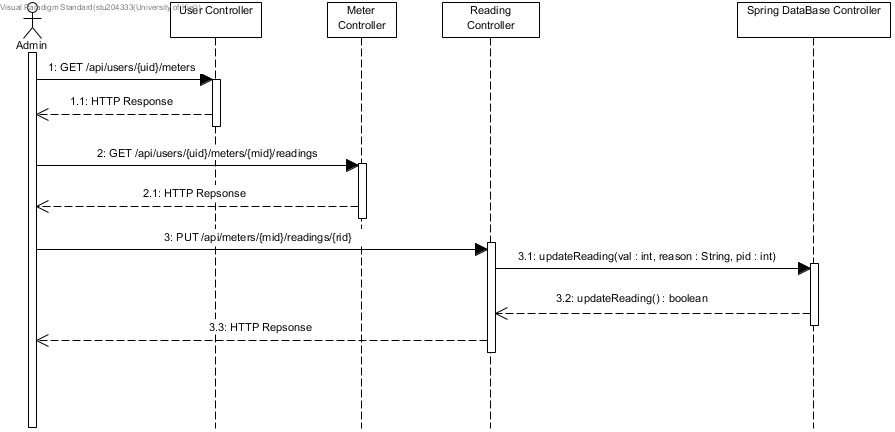
\includegraphics[width = 15cm]{img/diagrams/ChangeReading}
	\caption{Abfrage der Nutzerlisten}
\end{figure}
Administratoren können unter Angabe eines Grundes Zählerstände aktualisieren.
Dafür muss der Administrator zuerst mittels eines HTTP-Requests zu einer User-ID alle Zähler vom User Controller abfragen. Danach werden mittels einer weiteren Anfrage alle Zählerstände des Zählers abgefragt. Nun kann mittels eines PUT-Request mit der rid ein bestimmter Eintrag verändert werden. Dafür wird der neue Zählerstand, der Grund der Änderung und die ID des Admins versendet, die dann für den Funktionsaufruf ''updateReading'' verwendet wird. Wenn die Änderung erfolgreich war, sendet der Reading Controller in der HTTP Response einen Erfolg zurück.
	
	\chapter{Glossar}\label{chp:glossar}
	\thispagestyle{fancy}
	\begin{table}[h]
	\centering
	\begin{tabularx}{\textwidth}{X X}
		\rowcolor[HTML]{C0C0C0} 
		\textbf{Abkürzung} & \textbf{Beschreibung} \\
		Zähler & Bei einem Zähler handelt es sich um einen Gas-, Strom- oder Wasserzähler. Er misst den Verbrauch der jeweils namensgebenden Ressource. \\
		\rowcolor[HTML]{E7E7E7} 
		FAB (Floating Action Button) & Ein FAB ist ein Knopf, der in der unteren rechten Ecke einer Android-App sitzt und Zugriff zu essentiellen Funktionen ermöglicht. \\
		Administrator (Admin) & Der Administrator, vornehmlich ein Mitarbeiter von adesso energy, hat übergeordnete Zugriffsrechte, die es ihm erlauben, auf alle Daten zuzugreifen, sowie diese zu ändern. Er interagiert hierfür ausschließlich mit der Website. \\
		\rowcolor[HTML]{E7E7E7} 
		Benutzer (User) & Als Benutzer werden Kunden von adesso energy bezeichnet. Sie haben die Möglichkeit, über die App oder Website auf ihre Nutzerdaten zuzugreifen und aktuelle Zählerstände hochzuladen. Dabei bietet die App die Option, einen Zählerstand automatisch aus einem Bild zu erkennen. Der Benutzer kann sowohl mit der App als auch mit der Website interagieren. \\
		Web-Applikation & Der Server ist nicht Teil einer Web-Applikation. Aufgrund der umfassenden React-Architektur betrachten wir die Website als eigene Applikation. \\
		\rowcolor[HTML]{E7E7E7} 
		DTO (data transfer object) & Als data transfer objects bezeichnen wir die Objekte, die unsere Anwendungen über das HTTP-Protokoll übertragen. \\
		Paging & Durch paging  wird beschränkt, wie viele Daten ein Server auf einmal an einen Client versendet. 
	\end{tabularx}
	\caption{Glossar}
	\label{table:glossar}
\end{table}
	
	\bibliography{references}
	\pagenumbering{gobble} % Nummerierung deaktivieren
	
\end{document}
